\scanpage{7}
of the $(\varphi_i)$ (``Kummer structure'')
taking into account the actions
\tikz[baseline=0pt]{
  \node[inner sep=0pt] at (.10,.52) {\inserted{(16) and (18)}};
  \draw (-.62,-.12) .. controls (-.66,.26) and (-.48,.35) .. (-.20,.35)
    .. controls (.36,.35) and (.55,.27) .. (.78,.34);
}
of $\mathcal G_{X'}$
on $I$ and $\mathbf T(\overline{\mathbf Q})$. We can therefore
write
\[
(19)\qquad\mathcal G_{X'}\longrightarrow
\operatorname{Autext}\bigl(\pi_1(X'),\mathbf T(
\unsure{\tikz[baseline=-.4ex,x=1em,y=1em]{
  \draw (-.05,.87)--(.72,.89);
  \draw (.17,.64) .. controls (.03,.39) and (.03,.03) .. (-.10,-.38);
  \draw (.23,.30) .. controls (.46,.72) and (.78,.63) .. (.58,.24)
    .. controls (.42,-.04) and (.18,-.05) .. (.16,.20);
  \draw[line width=.65pt] (.10,.09) .. controls (.25,-.11) and (.43,.02) .. (.54,.18);
  \draw[line width=.65pt] (.23,.12)--(.20,-.16);
  \fill (.72,.34) circle (.035);
  \draw[line width=.65pt] (.62,.17)--(.64,-.16);
}}
),(\varphi_i)\bigr).
\]
\deleted{Suppose $X$}
% This looped trace may be a cancellation return; no additional word is supplied.
\unsure{\tikz[baseline=-.4ex,x=1em,y=1em]{
  \draw (-.30,.40)--(1.35,.40);
  \draw (-.55,.10)--(1.18,.10);
  \draw (.15,.30) .. controls (.87,.35) and (1.10,.29) .. (1.13,.15)
    .. controls (.94,.03) and (.84,.04) .. (.80,.10);
  \draw (.45,-.03) .. controls (.80,.03) and (1.03,-.05) .. (1.37,.02);
}}

Let $\widehat{\widetilde X'}$ be the normalization of
% Cancelled cluster above the live X; the underlying decoration remains uncertain.
$\overset{\unsure{\tikz[baseline=0pt,x=1em,y=1em]{
  \draw (0,.17) .. controls (.14,.42) and (.25,.07) .. (.43,.22)
    .. controls (.58,.40) and (.70,.11) .. (.82,.20);
  \draw[line width=.7pt] (-.03,.10)--(.34,.39)--(.09,.13)--(.48,.39)
    --(.22,.11)--(.69,.35)--(.45,.08)--(.89,.29);
  \draw[line width=.7pt] (.87,.18)--(.66,-.02)--(.84,-.08)--(.78,-.20);
}}}{X}$ in ``the extension''
defined by $\widetilde X'$, so we have a
profinite morphism
\[
\widehat{\widetilde X'}\longrightarrow X
\]
Let $\widetilde X'(I)$ be the inverse image of the set of
\deleted{generic} \inserted{maximal} points of the $D=\sum D_i$. We
therefore have
\[
(20)\qquad\widetilde X'(I)
\mathrel{\tikz[baseline=-.45ex,x=1em,y=1em]{
  \draw (0,0)--(1.80,0);
  \draw[line width=.65pt] (1.80,0) .. controls (1.82,.12) and (1.75,.15) .. (1.73,.035);
}}I
\]
and an action of $\deleted{\unsure{\mathcal G_{X'}|\mathcal G_X}}\mathcal E_{X'}$ on
$\widetilde X'(I)$ which transports \unsure{of|the} structure)
compatible with the actions on $I$
and the map (20). For $i\in I$) let
\[
(21)\qquad\widetilde X'(i)\subset\widetilde X'(I)
\]
be its fiber in $\widetilde X'(I)$,
% Physical cluster: on versus a leader end remains unresolved.
\unsure{\tikz[baseline=-.35ex,x=1em,y=1em]{
  \draw (.03,.04) .. controls (-.07,.22) and (.23,.27) .. (.16,.04)
    .. controls (.11,-.06) and (-.02,-.02) .. (.03,.04);
  \draw (-.08,.17)--(.12,.34);
  \draw (.20,.05) .. controls (.28,.23) and (.37,.18) .. (.37,.05)
    --(1.25,.01) .. controls (1.37,.01) and (1.41,-.02) .. (1.45,-.08);
}}
\margin{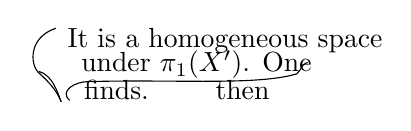
\begin{tikzpicture}[x=1em,y=1em]
  \node[anchor=west,inner sep=0pt] at (.35,1.75) {It is a homogeneous space};
  \node[anchor=west,inner sep=0pt] at (.85,.85) {under $\pi_1(X')$. One};
  \node[anchor=west,inner sep=0pt] at (.95,-.05) {finds.};
  \node[anchor=west,inner sep=0pt] at (5.70,-.05) {then};
  % Left parenthetical/enclosing curve, locally retraced at its lower turn.
  \draw (-.05,2.18) .. controls (-1.05,1.85) and (-1.00,.85) .. (-.65,.55)
    .. controls (-.15,.10) and (.02,-.18) .. (.14,-.48);
  \draw (-.66,.62) .. controls (-.18,.48) and (.01,-.12) .. (.14,-.48);
  % Continuing enclosure/attachment stroke; this does not delete the lower words.
  \draw (.45,-.43) .. controls (.05,-.08) and (.66,.25) .. (1.10,.25)
    .. controls (4.25,.34) and (7.20,.10) .. (8.65,.53)
    .. controls (8.83,.66) and (8.78,.86) .. (9.05,.94);
\end{tikzpicture}}
\mspage{6}
